\documentclass[prd,aps,10pt,nofootinbib,twocolumn,superscriptaddress,preprintnumbers,balancelastpage,longbibliography]{revtex4-1}

\usepackage{amsmath,amssymb}	
\usepackage{mathtools}
\usepackage{fontawesome}
\usepackage[dvipsnames]{xcolor}
\usepackage{hyperref}
\usepackage{xspace}
\usepackage{fancyhdr}
\usepackage{braket}
\usepackage{graphicx}
\usepackage{siunitx}
\usepackage{blindtext}
\usepackage{nicefrac}


\usepackage{afterpage}
\newcolumntype{L}[1]{>{\raggedright\let\newline\\\arraybackslash\hspace{0pt}}m{#1}}
\newcolumntype{C}[1]{>{\centering\let\newline\\\arraybackslash\hspace{0pt}}m{#1}}
\newcolumntype{R}[1]{>{\raggedleft\let\newline\\\arraybackslash\hspace{0pt}}m{#1}}
\usepackage{longtable}
\setlength{\LTcapwidth}{\textwidth}

\newcommand{\nbicon}{{\color{linkcolor}\faFileCodeO}\xspace}
\newcommand{\nblink}[1]{\href{https://github.com/smsharma/dark-photons-perturbations/blob/apr-2020/notebooks/#1.ipynb}{\nbicon}}
\newcommand{\githubmaster}{\href{https://github.com/smsharma/dark-photons-perturbations/}{\faGithub}\xspace}

\newcommand{\dd}{\mathrm{d}}
\newcommand{\mAp}{m_{A^\prime}}
\newcommand{\vect}[1]{\boldsymbol{\mathbf{#1}}}

\definecolor{deepgreen}{rgb}{0.2,0.8,0.2}
\newcommand{\SM}[1]{{\bf \color{deepgreen}{[SM: #1]}}}

\colorlet{linkcolor}{BrickRed}



\hypersetup{colorlinks=true,
linkcolor=linkcolor,
citecolor=linkcolor,
urlcolor=linkcolor,
,linktocpage=true
,pdfproducer=medialab}

\newcommand\hl[1]{{{\color{blue}(HL: #1)}}}

\DeclareSIUnit \h {\ensuremath{\mathit{h}}}
\DeclareSIUnit\electronvolt{e\kern-.05em V}
\DeclareSIUnit\parsec{pc}

\begin{document}

\title{Unveiling the Galactic Center $\gamma$-ray excess with neural simulation-based inference}
 
\author{Siddharth Mishra-Sharma}
\email{sm8383@nyu.edu}
\thanks{ORCID: \href{https://orcid.org/0000-0001-9088-7845}{0000-0001-9088-7845}}
\affiliation{Center for Cosmology and Particle Physics, Department of Physics, New York University, New York, NY 10003, USA}

\author{Kyle Cranmer}
\email{kyle.cranmer@nyu.edu}
\thanks{ORCID: \href{https://orcid.org/0000-0002-5769-7094]}{0000-0002-5769-7094]}}
\affiliation{Center for Cosmology and Particle Physics, Department of Physics, New York University, New York, NY 10003, USA}
\affiliation{Center for Data Science, New York University, 60 Fifth Ave, New York, NY 10011, USA}

\date{\today}

\begin{abstract}
Abstract will go here.
\end{abstract}

\maketitle

\section{Introduction}
\label{sec:intro}

\section{Analysis pipeline}
\label{sec:analysis}

\section{Results}
\label{sec:results}


%
\begin{figure*}
    \centering
    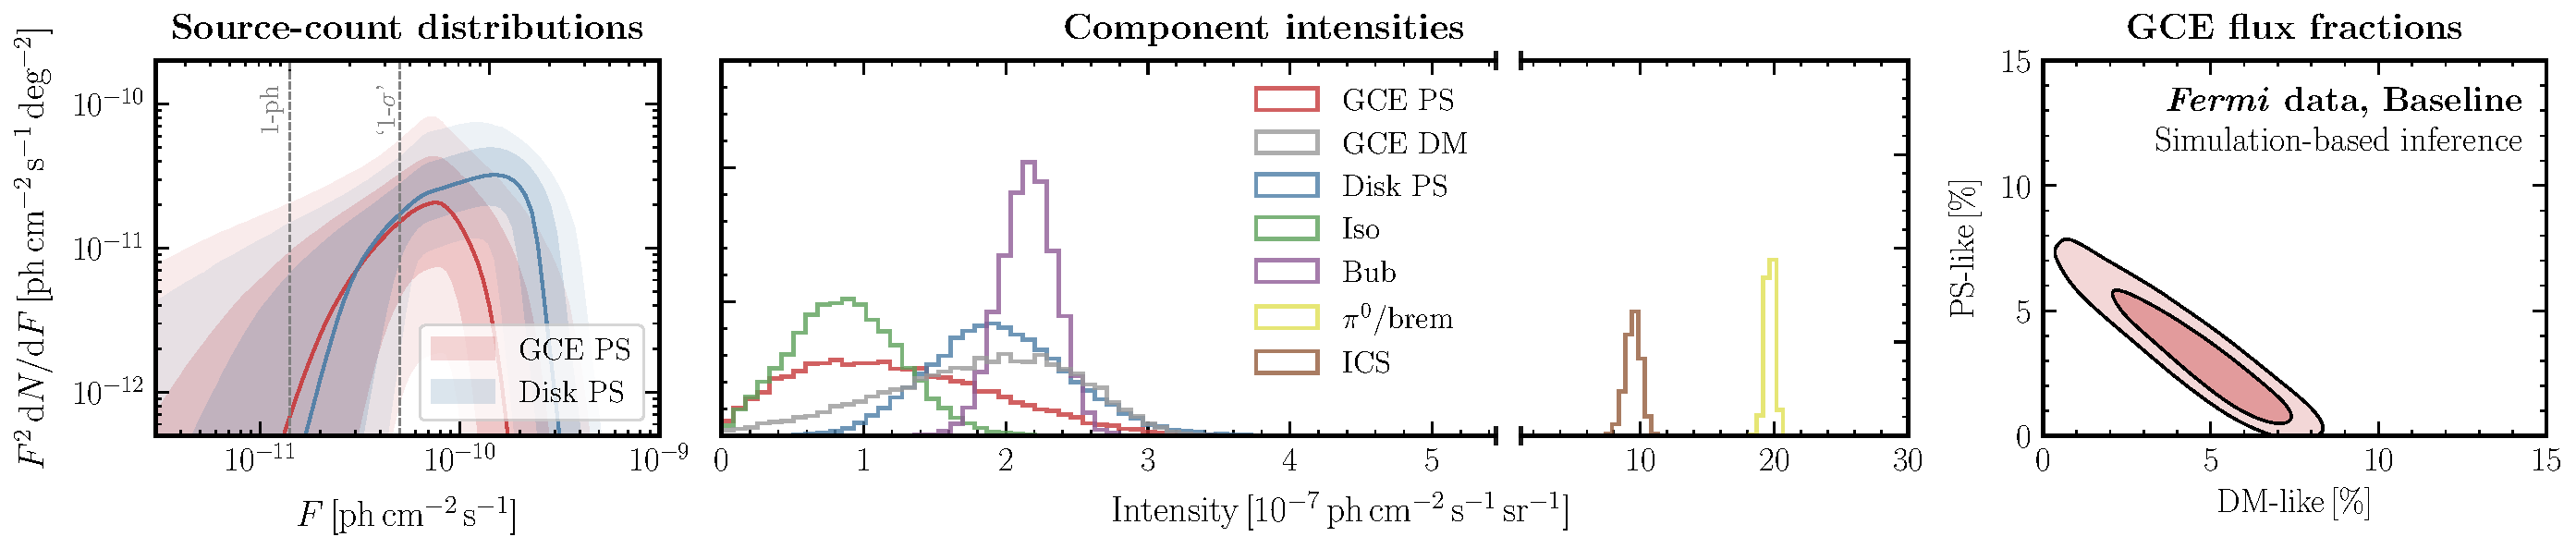
\includegraphics[width=0.95\textwidth]{plots/data_fid_sbi.pdf}
    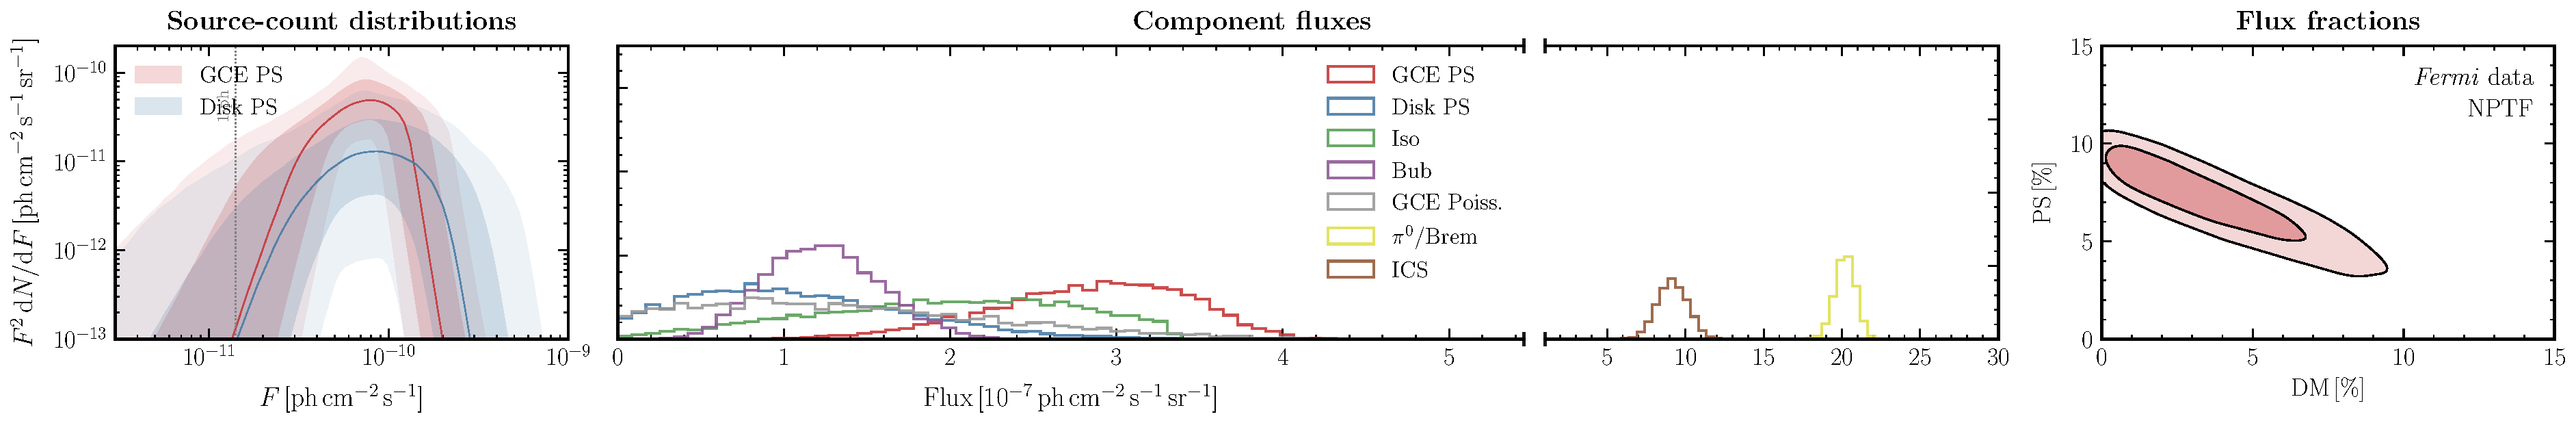
\includegraphics[width=0.95\textwidth]{plots/data_fid_nptf.pdf}
    \caption{Fiducial results on data.}
    \label{fig:fid_data}
\end{figure*}
%

\section{Susceptibility to mismodeling}
\label{sec:mismodeling}

\section{Foreground mismodeling}
\label{sec:fg-mismodeling}

\section{Signal mismodeling}
\label{sec:sig-mismodeling}

\section{Signal injection test}
\label{sec:sig-injection}


\section{Systematic variations on analysis}
\label{sec:systematics}

\section{Conclusions}
\label{sec:conclusion}

\vspace{.3cm}
%%%%%%%%%%%%%%%

\begin{acknowledgments}

We thank\ldots for helpful conversations.  
KC is partially supported by NSF awards ACI-1450310, OAC-1836650, and OAC-1841471, the NSF grant PHY-1505463, and the Moore-Sloan Data Science Environment at NYU. 
SM is supported by the NSF CAREER grant PHY-1554858, NSF grants PHY-1620727 and PHY-1915409, and the Simons Foundation. 
This work made use of the NYU IT High Performance Computing resources, services, and staff expertise. 
This research has made use of NASA's Astrophysics Data System. 
This research made use of the \texttt{astropy}~\cite{Price-Whelan:2018hus,Robitaille:2013mpa}, \texttt{IPython}~\cite{PER-GRA:2007}, Jupyter~\cite{Kluyver2016JupyterN}, \texttt{matplotlib}~\cite{Hunter:2007}, \texttt{NumPy}~\cite{numpy:2011}, \texttt{seaborn}~\cite{seaborn}, \texttt{pandas}~\cite{pandas:2010}, \texttt{SciPy}~\cite{2020SciPy-NMeth}, and \texttt{tqdm}~\cite{da2019tqdm}  software packages. 
\end{acknowledgments}

\appendix

\section{Systematics}
\label{app:systematics}

\section{Alternative summary statistics}
\label{app:summaries}

\bibliographystyle{apsrev4-1}
\bibliography{fermi-gce-sbi}

\end{document}
